\documentclass[a4paper]{article}

\usepackage[french]{babel}
\usepackage[T1]{fontenc}
\usepackage[utf8]{inputenc}
\usepackage{float}
\usepackage{amsmath}
\usepackage{graphicx}
\usepackage{wrapfig}
\usepackage{lscape}
\usepackage{rotating}
\usepackage{epstopdf}
\usepackage{multirow}
\usepackage{lmodern}
\usepackage[left=3cm, right=3cm, bottom=4cm, top=4cm]{geometry}
\usepackage{array}
\usepackage{pdfpages}
\usepackage{titlesec}



\usepackage[gen]{eurosym}
\DeclareUnicodeCharacter{20AC}{\euro{}}

\usepackage{hyperref}
\hypersetup{
    colorlinks,
    citecolor=black,
    filecolor=black,
    linkcolor=black,
    urlcolor=black
}

\title{Document de planification initiale}

\author
{
    François {\sc Boschet}\\
    Arnaud {\sc Lods}\\
    Marlène {\sc Tuekam}\\
    Alexandre {\sc Bouchet}\\
    Guillaume {\sc Perrudin}\\
    Nguyen {\sc Song Hai}\\
    Romain {\sc Colombat}
}

\date{\today}

\newcommand{\pagevierge}[0]{\newpage\thispagestyle{empty}\null\newpage}

\begin{document}
    % Ouh c'est sale.
    \hypersetup{pageanchor=false}
    
\includepdf[pages=1]{figure/couv.pdf}
    \hypersetup{pageanchor=true}

    \newpage
    \thispagestyle{empty}
    \mbox{}

    \newpage
    % A decommenter pour la release
    \setcounter{tocdepth}{4}
    \tableofcontents
    \setlength{\parskip}{10pt}

    \newpage
    \thispagestyle{empty}
    \mbox{}

    \newpage
    
    
    \section{Introduction}

	\section{Rappel de la phase d'analyse}
\label{sec:rappel}
	
	\section{Phase de conception}
	
	\section{Phase de développement}
\label{sec:dev}

	Afin d'obtenir des retours sur l'application et d'adapter notre développement ou de corriger certaines fonctionnalités, nous avons donc décidé de découper la phase de développement en différentes itérations pour réaliser plusieurs livrables. Ces livraisons précéderont une série de tests d'intégration pour vérifier et corriger la présence de bugs, et un temps de développement est prévu afin de prendre en compte les remarques et les retours sur la version livrée et adapter l'application. Les tests unitaires, réalisés pour vérifier le fonctionnement de chaque tâche, ne sont pas détaillés et sont compris dans les durées des tâches décrites par la suite, vous pouvez cependant retrouver le détail de ceux-ci dans le diagramme de Gantt à la fin du rapport. Nous avons pris en considération des durées de test allant de 50\% à 100\% de la durée de la tâche, suivant la complexité de celle-ci.

	Nous avons décidé de découper le projet en trois itérations. Les deux premières représentent les deux grosses fonctionnalités primordiales, mais aussi les plus complexes, à réaliser. Lors de la première itération, nous fournirons le moteur de recherche de celle-ci, ainsi qu'une base de données contenant des jeux de tests. Cela permettra de vérifier le bon fonctionnement de la première partie du site, et de confirmer qu'elle correspond bien à ce qui est attendu. La version de la seconde itération, dans la continuité de la première, contiendra en plus la page de consultation d'un document, avec toutes les fonctionnalités liées. Cette page étant la partie centrale du site, il est nécessaire de rendre celle-ci en milieu de phase de développement pour avoir le temps d'y apporter des modifications. Enfin, la dernière itération contiendra toutes les fonctionnalités annexes; c'est-à-dire la gestion d'utilisateurs, la gestion des revues de presse et la page d'accueil. Celle-ci sera rendue peu de temps avant la livraison finale, pour permettre d'apporter quelques dernières modifications si le besoin s'en fait ressentir.

	En résumé, voici comment se déroulera la phase de développement :

	\begin{figure}[H]
        \centering
        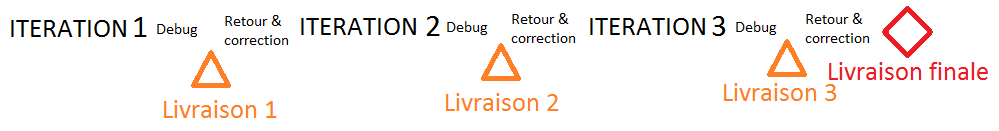
\includegraphics[width=\textwidth]{figure/schema_developpement.png}
            \caption{Schéma représentant la phase de développement}
            \label{fig:sch_dev}
    \end{figure}
    \section{Itération 1 : Moteur de recherche}

	\subsection{La recherche} 
		La première étape de la mise en place de la recherche est la configuration d'Elasticsearch. C'est lui qui fera la recherche au sein de la base. Cependant, il est nécessaire qu'il puisse communiquer avec la base de données MongoDB afin d'en récupérer le contenu. Elasticsearch dispose d'ailleurs d'un plugin qui lui permet de se lier à une base de données et de mettre à jour son index lors d'ajouts ou de modifications de la base. Elasticsearch sera alors capable de gérer une recherche d'articles, de journaux ou de revues de presse. Cette étape est la tâche principale. Ensuite, il faudra implémenter la communication entre Elasticsearch et l'interface utilisateur. C'est-à-dire une recherche faite par l'utilisateur à partir de l'application sera transmise à Elasticsearch et les résultats seront retournés à l'utilisateur.

		\begin{itemize}
			\item configuration d'Elasticsearch et de MongoDB : 10h
			\item communication entre l'interface et Elasticsearch : 4h
		\end{itemize}

	\subsection{Critères et filtres de recherche} 
		Elasticsearch est capable de gérer les recherches avec des critères ainsi que de trier les résultats obtenus. Il suffira donc d'implémenter l'interface utilisateur pour l'utilisation de ces critères et d'envoyer ceux qui ont été choisis à Elasticsearch. Pour les filtres, c'est le même procédé. Les deux étapes prendront 3h chacune.

		\begin{itemize}
			\item critères de recherche : 3h
			\item filtres de recherche : 3h
		\end{itemize}

	\subsection{Affichage des résultats} 
		Les résultats de la recherche ne se résument pas seulement à une liste d'articles. Suivant le document recherché, de nombreuses informations reliées à ceux-ci seront affichées; pour un article il y aura le titre, l'auteur, les tags, le journal, la date, le contenu, et son appartenance ou non à une revue de presse. Pour afficher ces informations, il faudra questionner la base de données pour obtenir celles-ci ou les demander à Elasticsearch. Il faudra ensuite afficher ces résultats, puis adapter ce qui a été fait pour un type de document pour les deux autres types de document.

		\begin{itemize}
			\item récupération et traitement des informations pour un document : 8h
			\item affichage des résultats : 4h
			\item adaptation pour les autres types de document : 4h
		\end{itemize}


    \section{Itération 2 : Consultation de documents}

	\subsection{Consulter}
		Après avoir développé le moteur de recherche, nous entrerons dans la mise en place des fonctionnalités liées à la page de consultation de documents. Comme nous l'avions énoncé dans le rapport de spécifications, trois modes de consultation seront proposés; article, journal et revue de presse. Trois objectifs sont définis pour cette consultation; consulter, informer et guider le lecteur.


		Tout d'abord, nous allons mettre en place une visionneuse de documents, Openseadragon. C'est une visionneuse d'image haute définition adaptée à notre projet dans la mesure où elle permet d'ajouter des overlays pour de nouvelles fonctionnalités (boutons de navigation, polygones délémiteurs, zoom, calques, ...). Cette étape de développement et de tests est estimée à 24h.

		Ensuite nous rajouterons une fonctionnalités de recherche dans le document à la visionneuse (5h).

	\subsection{Informer}
		Puis vient l'implémentation des fonctionnalités d'information. Il est question ici :
		Dans un premier temps, de développer une interface permettant à l'utilisateur de rajouter des informations au document. Il s'agit notamment de :
			\begin{itemize}
			\item Gestion des tags (10h)
			\item ajout à une revue de presse ou aux favoris (10h)
			\end{itemize}

		Dans un second temps, il est question de réaliser une architecture du document : interroger la base de données afin de revueillir toutes les informations importantes liées au document consulté. Les informations affichées pourront être par exemple le titre, la date d'un journal, les articles associés, le titre d'un aticle, les tags... Cette tâche nécessitera 8h de travail.

	\subsection{Guider}
		En dernier lieu, nous allons développer les fonctionnalités de guidage.
		Parcours d'une revue de presse (8h)
		Proposition d'articles similaires, des revues de presse de même thématique (10h)

		À l'issue du développement de toutes ces fonctionnalités, nous réaliserons des test d'intégration estimés à 20h de travail.
    \section{Itération 3 : Revue, utilisateur et accueil}
\label{subsec:revue_util_accueil}
	\subsection{Revue de presse}
	\label{subsec:revue}

		L'architecture des revues de presse aura été développé avant dans le cadre du moteur de recherche - puis de la consultation de document -, et la prochaine étape sera de créer leur page spécifique. Il sera donc nécessaire de réaliser l'interface permettant de créer de nouvelles revues de presse, puis de créer une page qui permettra de visualiser une revue de presse créer, et de modifier celle-ci.

		\begin{itemize}
			\item page résumé et modification revue de presse : 6h
			\item page ajout revue de presse : 3h
		\end{itemize}

	\subsection{Page d'accueil}
	\label{subsec:accueil}
		\subsubsection{Interface graphique}
		\label{subsubsec:acc_interface}
			
			La page d'accueil permettant à l'utilisateur de comprendre le site, on réalisera une interface graphique simple et fonctionnelle orientant l'utilisateur vers les fonctions de base du site, c'est-à-dire la recherche d'articles, journaux ou revues de presse et leur visionnage. L'affichage d'articles vedettes complètera l'accompagnement de l'utilisateur en lui proposant des articles susceptibles d'intéresser un maximum de public.
			Le site web disposera d'une interface graphique au design moderne, fonctionnel et minimaliste. Le design se verra aussi cohérent entre les différentes pages du site. Le Framework CSS Bootstrap nous permettra de développer une plateforme qui s'adaptera à tout type de support.

			\begin{itemize}
				\item interface et architecture de la page : 8h
			\end{itemize}

		\subsubsection{Formulaire de recherche dans la base}
		\label{subsubsec:acc_rech}
			Pour la partie de recherche intégrée à la page d’accueil, celle-ci comportera un formulaire de recherche texte et une liste déroulante permettant de choisir le type de document pour la recherche dans la base (articles, journaux, revue de presse). Ce formulaire reprendra les éléments de recherche développés avec le moteur de recherche de l'itération 1, et sera donc plutôt rapide.

			\begin{itemize}
				\item formulaire de recherche simple : 1h
			\end{itemize}

		\subsubsection{Affiche des articles vedettes} 
		\label{subsubsec:acc_article}
			Nous définirons un critère de choix des articles et des revues de presse susceptibles d'intéresser le nouveau visiteur. Les documents seront sélectionnés sur la base de données et affichés sur la page d'accueil sous forme de miniatures avec les informations récupérées.

			\begin{itemize}
				\item sélection articles et revues de presse : 5h
				\item génération des éléments HTML : 1h
			\end{itemize}

	\subsection{Gestion d'utilisateur}
	\label{subsec:utilisateur}
		\subsubsection{Inscription et connexion}
		\label{subsubsec:util_inscr}
			Pour pouvoir gérer les utilisateurs, il faut créer des utilisateurs. On va faire une page de l’inscription pour les utilisateurs qui veulent s’inscrire. Les principaux éléments dans cette page sont des champs d’informations personnelles de l’utilisateur: nom, pseudo, mot de passe, email, etc … Il sera donc nécessaire de créer la page et le formulaire d'inscription d'utilisateurs, et de confirmer l'inscription par l'envoie d'un mail de confirmation. Un espace de connexion devra aussi être créé à partir de la page d'accueil, et un espace lui permettant de récupérer un nouveau mot de passes s'il a oublié le sien. Un mail de vérification, et une page dédiée au changement d'un mot de passe sera créé.

			\begin{itemize}
				\item inscription d'utilisateur : 4h
				\item espace de connexion : 1h
				\item réinitialisation de mot de passe : 2h
			\end{itemize}

		\subsubsection{Profil utilisateur}
		\label{subsubsec:util_profil}
			La tâche suivante constituera à développé l'espace personnel d'un utilisateur. Il faudra travailler sur une page lui permettant de modifier ses paramètres (mail, mot de passe). Ensuite, sur cette page il sera nécessaire de créer trois listes qui contiendront respectivement les revues de presse qu'il a créé, celles auxquelles il a contribué et ses favoris. Les requêtes dans la base de données seront donc établies, et on reprendra le système de gestion d'une revue de presse pour les favoris.

			\begin{itemize}
				\item espace de paramétrage : 2h
				\item revues de presse et favoris : 5h
			\end{itemize}
    
    \section{Planification du projet}
\label{sec:orga}

	Les différents délivrables du projet 4INFO imposent une gestion de projet suivant un modèle de cycle en V. Cependant, nous sommes libres d'adapter nos propres méthodes de développement 

	Ici, nous avons de nombreuses fonctionnalités que nous allons être amené à réaliser. Il est donc nécessaire de penser à une bonne méthode de gestion lors du développement. Cela nous permettra de gérer au mieux le temps qui nous est imparti en prenant en compte les ressources que nous avons à disposition notamment humaines. D'un côté, il est nécessaire d'évaluer l'importance de chaque fonctionnalité, définie bien précisément, et de l'autre, la partie la plus complexe, il nous faut estimer la durée pour réaliser chaque tâche.

	En respectant un modèle de cycle en V, nous nous retrouverions donc à développer la plateforme, puis à effectuer différentes séries de tests avant de la délivrer. Le problème de cette méthode est que nous allons devoir faire une sélection de fonctionnalités à développer, s'y tenir, et un livrable ne sera fournit qu'à la fin. Entre autre, nous ne pourrons avoir un retour sur l'application que lorsque le développement sera fini. Il sera impossible d'inférer sur les fonctionnalités puisqu'il n'y aura aucun retour durant le temps de développement. 

	C'est pourquoi nous pensons planifier le développement de l'application en se basant sur les méthodes agiles. Nous aurons donc une liste de fonctionnalités, triée suivant leur importance et leur difficulté à être développées. En considérant les ressources mises à disposition, nous délivrerons et effectuerons en continue des tests pour chacune des fonctionnalités. Ainsi il sera possible de présenter l'avancement au milieu du projet à nos encadrants, et il serait possible de redéfinir certaines priorités pour les fonctionnalités restantes, ou en rajouter par la suite si nous prenons de l'avance sur le développement. Si celles-ci se trouvent être plus intéressantes (ou plus faciles), nous pourrions nous retrouver à les développer en priorité par rapport à des fonctionnalités définies avant. Enfin, cela permet à un instant T d'avoir un produit fonctionnel.

	En faisant une liste non exhaustive de tâches globales (on ne détaille pas encore toutes les sous-tâches de développement qu'une tâche implique, et les tests sont inclus dans le temps de la tâche), et en les ordonnant de manière à obtenir une plateforme qui contiendra au fur et à mesure de plus en plus de fonctionnalités en partant des plus importantes; on arrive à ce schéma de planification.

	\begin{figure}[H]
        \centering
        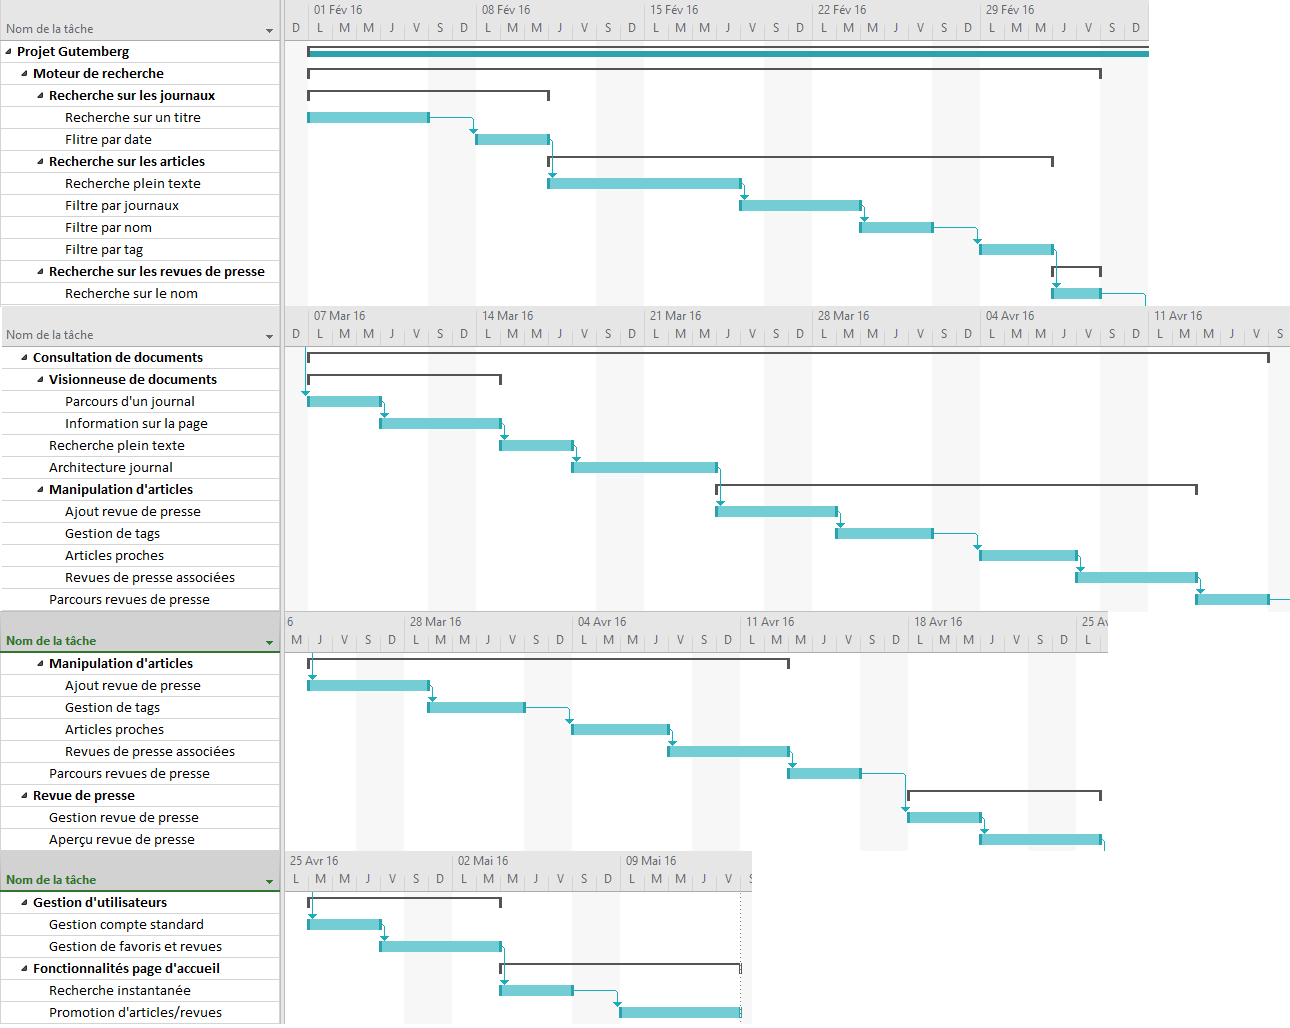
\includegraphics[width=1.3\textwidth, angle=90]{figures/plan.png}
            \caption{Plannification}
            \label{fig:plan_recherche}
    \end{figure}

	\section{Conclusion}
\label{sec:conclusion}
	
	Ce rapport et les deux présentations qui donnent suite à ce dernier représentent la fin de la phase d'analyse et de spécifications. Nous avons vu et estimé la durée de chacune des tâches pour chaque itération du projet. Cela nous a permis d'établir une planification initiale des tâches pour le reste du projet, du début de la phase de conception jusqu'au rendu de la dernière version du projet.

	L'étape suivante du projet sera donc la phase de conception de celui-ci. Nous établirons l'architecture de la base de données que nous utiliserons, nous définirons les différents modules de l'application, et la façon dont ceux-ci communiquent entre eux, et nous procéderons à l'installation de l'environnement de travail pour la suite du projet.
	
	\newpage
	\section{Annexes}
\label{sec:annexes}

	\begin{figure}[H]
        \centering
        
\includegraphics[width=\textwidth]{figure/gantt.png}
            \caption{Partie diagramme de Gantt}
            \label{fig:gantt}
    \end{figure}

    \begin{figure}[H]
        \centering
        
\includegraphics[width=\textwidth]{figure/gantt.png}
            \caption{Partie diagramme de Gantt}
            \label{fig:gantt}
    \end{figure}

    \begin{figure}[H]
        \centering
        
\includegraphics[width=\textwidth]{figure/gantt.png}
            \caption{Partie diagramme de Gantt}
            \label{fig:gantt}
    \end{figure}
	
	\bibliographystyle{plain}
    \bibliography{input/biblio}
    
    
    % Manoucherie incoming
    \pagevierge
    \ifthenelse{\isodd{\thepage}}
    {\pagevierge}
    {}
    
\includepdf[pages=2]{figure/couv.pdf}
    
    
\end{document}
